%------------------------------------------------------
\chapter{Deep Reinforcement Learning}

\section{Getting Started}

From Lex Fridman's intro lecture on deep reinforcement learning \href{https://youtu.be/zR11FLZ-O9M?t=0}{[video]}.

Deep reinforcement learning (RL) is perhaps one of the most exciting fields in artificial intelligence (AI). It marries the beauty and power of deep neural networks to represent and comprehend the world with the ability to act on that understanding. That's basically what the creation of intelligent beings is. Recent breakthroughs in RL captivate our imagination and inspire us.  

RL at high level: An agent has to make a sequence of decisions. 

\paragraph*{Types of Learning:}
4 learning domains within machine learning: Supervised, semi-supervised, unsupervised, and reinforcement. People often think that supervised learning is the only domain that requires manual labeling, however in reality, all types of machine learning are "supervised" in some way by a loss function. Every type of machine learning is supervised learning to a degree. These names for the domains tell us about the cost of human labor required to obtain that supervision.
\begin{itemize}
	\item Supervised learning: "teach by example"; RL: "teach by experience"
\end{itemize}

\paragraph*{RL in humans: }
Humans appear to learn to walk (and do many other activities) through "very few examples" of trial and error. \textbf{How} is an open question. Possible answers: 
\begin{itemize}
	\item Hardware: 230 million years of bipedal movement data
	\item Imitation learning: Observation of other humans walking
	\item Algorithms: Better than backpropagation and stochastic gradient descent
\end{itemize}

Current spot: \url{https://youtu.be/zR11FLZ-O9M?t=757}


\subsection*{3 Types of RL}
There are countless ways to taxonomize all of the reinforcement learning algorithms. At the highest level, there are model-based algos and model-free algos. We generally put algorithms under 3 categories: model-based, value-based, and policy-based. 

\paragraph*{Model-based: }
\begin{itemize}
	\item Learn a model of the world, then plan using the model. As an agent interacts with the environment, it constructs a model for what the dynamics of the world might be. 
	\item Better sample efficiency. Once you have a model, you can do all kinds of reasoning that doesn't require experiencing each scenario.  
	\item In chess and in Go, the model is given to you. The agent knows the rules of the game. 
\end{itemize}

\begin{quest}
	\item What is meant by ``model" is model-based learning? 
	\begin{ans}
		In this context,  a model of the environment would be a function which predicts state transitions and rewards.
	\end{ans}
	
	\cloze AlphaZero is the reinforcement learning algorithm that learned to play Chess and Shogi. 

	\cloze AlphaZero is a famous example of a model-based algorithm. 

	\href{https://arxiv.org/pdf/1712.01815.pdf}{[AlphaZero paper, 2017]}

	\item If model-based methods are more sample efficient when they work, what is the advantage of model-free methods?
	\item \cloze Q-functions are also called action-value functions. 
	
	\item And what's te difference between action-value function and state-value function?
	\begin{ans}
		THe state-value function returns the value of achieving a certain state, whereas the action-value function returns the value for choosing an action in a state. 
	\end{ans}
	
	\item Why are Q-functions sometimes called action-value functions?
	\begin{ans}
		Because the Q-function gives us the value for taking an action in some state. 
	\end{ans} 
\end{quest}

Note that, as of 2018, model-free methods are more popular and have been more extensively developed and tested than model-based methods.


\paragraph*{Value-based: } 
\begin{itemize}
	\item Learn the state or state-action value. Value-based methods look to estimate the quality of states and the possible actions performed in them. This quality of the state is then used to pick a ``best'' action. 
	\item Act by choosing the best action in a state. This is considered indirect learning of a ``policy''.
\end{itemize}  

\paragraph*{Policy-based: }
\begin{itemize}
	\item Learn the stochastic policy function that maps state to action.
	\item Directly learn a policy function. In other words, take as input the representation (or representation of that world) and output an action. This action will be stochastic. 
	\item Act by sampling policy. 
	\item Exploration is baked in. Why? The output action is stochastic, meaning it's a r.v. 
\end{itemize}


Great resource for learning about deep reinforcement learning: Open AI Spinning Up \href{https://spinningup.openai.com/en/latest/user/introduction.html}{[link]}





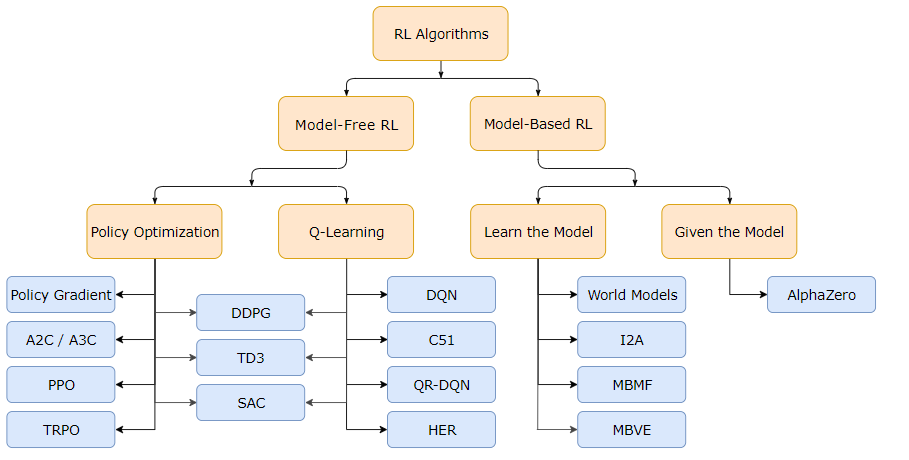
\includegraphics[width=0.9\linewidth]{rl_algos_taxonomies}

\section{Review Paper: }

\cite{arulkumaran2017deep}

Deep learning is enabling reinforcement learning (RL) to scale to problems that were previously intractable, such as learning to play video games directly from pixels.  Deep reinforcement learning algorithms are also applied to robotics, allowing control policies for robots to eb learned directly from camera inputs in the real world. 
\paragraph*{Topics covered: }Value-based methods, policy-based methods, central algorithms in deep reinforcement learning such as the deep Q-network, trust region policy otpimisation, and asnchronous advantage actor-critic. Conclude with several current areas of research within the field. 

Primary goal of the field of artificial intelligence (AI) is to produce fully autonomous agents that interact with their environments to learn optimal behaviours, improving over time through trial and error. Reinforcement learning is a principled mathematical framework for experience-driven autonomous learning. RL is a general way of approaching optimisation problems by trial and error.

The most important property of deep learning is that deep neural networks can automatically find compact low-dimensional representations (features) of high-dimensional data (e.g., images, text and audio) 


the use of
deep learning algorithms within RL defining the field of
“deep reinforcement learning” (DRL)

For a more comprehensive survey of recent efforts in
DRL, including applications of DRL to areas such as natural
language processing [106, 5], we refer readers to the overview
by Li [78]


The first, kickstarting the revolution in DRL,
was the development of an algorithm that could learn to play
a range of Atari 2600 video games at a superhuman level,
directly from image pixels [84]. Providing solutions for the
instability of function approximation techniques in RL, this
work was the first to convincingly demonstrate that RL agents
could be trained on raw, high-dimensional observations, solely
based on a reward signal. The second standout success was
the development of a hybrid DRL system, AlphaGo, that
defeated a human world champion in Go [128], paralleling the
historic achievement of IBM’s Deep Blue in chess two decades
earlier [19] and IBM’s Watson DeepQA system that beat the
best human Jeopardy! players [31].


AlphaGo
was composed of neural networks that were trained using
supervised and reinforcement learning, in combination with
a traditional heuristic search algorithm


In a step towards even more capable agents,
DRL has been used to create agents that can meta-learn (“learn
to learn”) [29, 156], allowing them to generalise to complex
visual environments they have never seen before

One of the
driving forces behind DRL is the vision of creating systems
that are capable of learning how to adapt in the real world.




\section{Mine}


\subsection*{\href{https://en.wikipedia.org/wiki/-learning}{Q-learning}}
\begin{quest}
	\item \cloze Q-learning is a model-free RL algorithm.
	
	\cloze Q-learning gets is name because the agent learns the quality of actions to know how to act. 

	\cloze In Q-learning, "Q" function is computed to maximize expected rewards for an action taken in a given state.  
	
	\cloze "Model-free" means that an agent does not require a model of the environment.
	
	\cloze For set of states $S$ and set of actions $A$, the Q-function is a map s.t. $Q:S\times A\to \mathbb{R}$.
	
	\item In Q-learning, $Q$ is updated according to 
	$$ Q_{\text{new}}(s, a) := Q(s, a) 
		+ \alpha \cdot 
			\left( r + \gamma \max_{a_b\in A} Q(s', a_b) 
			- Q(s, a) \right) $$.
	\begin{itemize}
		\item $Q(s, a)$: The "quality" fn. at the current state $s$
		\item $\alpha$: The learning rate. $0 \leq \alpha \leq 1$. Values close to 1 make faster changes to $Q$.  
		\item $r$: Reward received when moving from $s \to s'$
		\item $\gamma$: The discount factor. Quantifies how much to "discount" the 
		\item $\max_{a_b\in A} Q(s', a_b)$: Estimate of optimal future Q-value. This would be the highest $Q(s'|a_b)$, where $a_b$ is the "best" action and $s'$ is the next state.  
	\end{itemize}
\end{quest} 



\section{DQN }
\cite{mnih2015human}

\section{Collection of Refs}

Deep Attention Recurrent Q-Network. 2015. \cite{sorokin2015deep}  




\url{https://causalai.net/r26.pdf}

\href{https://paperswithcode.com/methods/area/reinforcement-learning}{Papers with Code - RL}

\href{https://paperswithcode.com/task/representation-learning}{Papers with Code - Representation Learning}

\href{https://paperswithcode.com/paper/near-optimal-representation-learning-for}{	Near-Optimal Representation Learning for Hierarchical Reinforcement Learning}

\href{https://arxiv.org/pdf/1911.08265.pdf}{Mastering Atari, Go, Chess and Shogi by Planning with a Learned Model, 2020}

"... deep RL algorithm based on the
maximum entropy reinforcement learning framework. In this framework, the actor aims to maximize expected reward while also maximizing entropy. That is, to succeed at the task while acting as randomly as possible" - \href{https://arxiv.org/pdf/1801.01290.pdf}{Soft Actor-Critic: Off-Policy Maximum ENtropy Deep RL w/ a Stochastic Actor} 


% --------------------------------------------
\chapter{Attention Mechanism}




\href{https://proceedings.neurips.cc/paper/2017/file/3f5ee243547dee91fbd053c1c4a845aa-Paper.pdf}{Attention is All You Need, 2016}

\href{https://arxiv.org/pdf/2009.14794.pdf}{Rethinking Attention with Performers}

\section{Image + Attention}
\subsection{Facebook AI Research applies Transformer architecture to streamline object detection models. 2020.}
\begin{itemize}
	\item Tags:
	\item Affiliations: Facebook AI
	\item \href{https://ai.facebook.com/research/publications/end-to-end-object-detection-with-transformers}{[paper]}
	\item \href{https://venturebeat.com/2020/05/28/facebook-ai-research-applies-transformer-architecture-to-streamline-object-detection-models/}{[article]}  
\end{itemize}

\subsection{Attention Agent: Neuroevolution of Self-Interpretable Agents. Tang, Ngyuen, and Ha. 2020.} 
\begin{itemize}
	\item Tags: interpretability, evolutionary algorithm, transformer, self-attention, deep RL, image input
	\item Affiliations: Google Brain, Google Japan
\end{itemize}



\subsection{CURL: Contrastive Unsupervised Representations for Reinforcement Learning. Srinivas et al., 2020.}
\begin{itemize}
	\item Tags: unsupervised, representation learning, deep RL, CNN, image input
	\item Affiliations
\end{itemize}

\subsection{M-CURL: Masked Contrastive Representation Learning for Reinforcement Learning. Zhu et al., 2020.}
\begin{itemize}
	\item Tags: masked training, representation learning, sample efficiency, self-supervised, CNN, transformer, deep RL, BERT, contrastive learning, image input
	\item Affiliations: 1. Uniersity of Science an Technology of China. 2. Microsoft Research
\end{itemize}

Improving sample efficiency is a key research problem in reinforcement learning (RL). Contrastive Unsupervised representations for Reinforcement Learning (CURL).


\begin{quest}
	\item Besides the involvement masked training, what's the key difference between M-CURL and CURL?
	\begin{ans}
		M-CURL deals with videos (seqs of images) rather than individual images. Although consecutive frames are highly correlated, CURL handles them independently. M-CURL's main improvement, outside of getting improved performance on several benchmarks, is that it takes into consideration the correlation between sequential frames.  

		This is where the transformer comes in. The Transformer, together with a CNN encoder, leverages the correlation of consecutive input frames to reproduce missing features in masked frames.  
	\end{ans}
	
	\item Why use Transformers, specifically?
	\begin{ans}
		The input in this paper was a sequence of images rather than a single image. Transformers (Waswani et al., 2017) are the current state-of-the-art module for modeling sequences and capturing their interdependencies.  
	\end{ans}

	\item The authors call the Transformer module an "auxilliary Transformer". What makes it auxiliary? 

	\item CNN encoder of what? What's being encoded? And what is meant by "encode" here?
	\begin{ans}

	\end{ans}

	\item Why discard the Transformer during action selection?

	\item Policy network? What does it do? What is it made up of? What are its inputs?

	\item Contrastive learning?
\end{quest}


%------------------------------------------------------
\chapter{Generative Adversarial Networks}



\subsection{GANs \cite{goodfellow2014generative}}

\subsection*{Abstract \& Introduction}

\paragraph*{Abstract: } Goodfellow et al. propose a new framework for estimating generative models via an adversarial process, in which two models are simultaneously trained:
\begin{itemize}
\item
	$G$: a generative model that captures the data distribution, and
\item
	$D$: a discriminative model that estimates the probability that a sample came from the training data rather than $G$
\end{itemize}
The training procedure for $G$ is to maximize the probability of $D$ making a mistake. This framework corresponds to a minimax two-player game. In the space of arbitrary functions $G$ and $D$, a unique solution exists, with $G$ recovering the training data distribution and $D$ equal to \texttt{$\frac{1}{2}$} everywhere. In the case where $G$ and $D$ are defined by multilayer perceptrons, the entire system can be trained with backpropagation. There is no need for any Markov chains or unrolled approximate inference networks during either training or generation of samples.


\paragraph*{Introduction: }

In the proposed adversarial nets framework, the generative model is pitted against an adversary: a discriminative model that learns to determine whether a sample is from the model distribution or the data distribution.
\begin{itemize}
\item \textbf{Counterfeiters Analogy: } The generative model can be thought of as analogous to a team of counterfeiters, trying to produce fake currency and use it without detection, while the discriminative model is analogous to the police, trying to detect the counterfeit currency. Competition in this game drives both teams to improve their methods until the counterfeits are indistiguishable from the genuine articles.
\end{itemize}
In this article, we explore the special case when the generative model generates samples by passing random noise through a multilayer perceptron, and the discriminative model is also a multilayer perceptron. We refer to this special case as adversarial nets. In this case, we can \textbf{train both models using only the highly successful backpropagation and dropout algorithms} [17] and sample from the generative model using only forward propagation.

\subsubsection*{Adversarial Net Algorithm}
The adversarial modeling framework is most straightforward to apply when the models are both multilayer perceptrons. To learn the generator’s distribution $p_g$ over data $\bm{x}$, $p_g(\bm{x})$, we define a prior on input noise variables, $p_{\bm{z}}(\bm{z})$, then represent a mapping to data space as $G(\bm{z}| \theta_g)$, where $G$ is a differentiable function represented by a multilayer perceptron with parameters $\theta_g$. We also define a second multilayer perceptron $D(\bm{x} | \theta_d)$ that outputs a single scalar. $D(\bm{x})$ represents the probability that $\bm{x}$ came from the data rather than $p_g$. We train $D$ to maximize the probability of assigning the correct label to both training examples and samples from $G$. We simultaneously train $G$ to minimize $ \log(1 - D(G(\bm{z})))$. In other words, $D$ and $G$ play the following two-player minimax game with value function, $V(G,D)$:
\[
	\min_G\max_D V(D,G) =
	\mathbb{E}_{\bm{x}\sim p_{\text{data}}(\bm{x})}
	\left[ \log D(\bm{x}) \right]
	+
	\mathbb{E}_{\bm{x}\sim p_{\bm{z}}(\bm{z})}
	\left[ \log\left( 1 - D(G(\bm{z})) \right) \right].
\]

Goodfellow et al. present a theoretical analysis of adversarial nets, essentially showing that the training criterion allows one to recover the data generating distribution as $G$ and $D$ are given enough capacity, i.e., in the non-parametric limit.

Figure 1 explains this approach: GANs are trained by simultaneously updating the discriminative distribution, $D$, so that it discriminates between samples from the data generating distribution, $p_{\bm{x}}$, and those of the generative distribution $p_g$ (G).

After several steps of training, if $G$ and $D$ have enough capacity, they will reach a point at which both cannot improve because $p_g=p_{\text{data}}$. The discriminator is unable to differentiate b/w the two distributions, i.e. \texttt{$D(\bm{x})=\frac{1}{2}$} .


\begin{algorithm}[H]
\SetAlgoLined
\caption{Minibatch SGD training of GAN. The number of steps to apply the discriminator, $k$, is a hyperparameter. $k=1$ is the least expensive option.}


\For{number of training iterations}{
	\For{$k$ steps}{
		\# Apply discriminator
		\begin{itemize}
		\item
			Sample minibatch of $m$ noise samples
			$\{ \bm{z}^{(1)},\ldots, \bm{z}^{(m)} \}$ from noise prior, $p_g(\bm{z})$.
		\item
			Sample minibatch of $m$ examples
			$\{ \bm{x}^{(1)},  \ldots, \bm{x}^{(m)} \}$ from data generating distribution, $p_{\text{data}}(\bm{x})$.
		\item
			Update the discriminator by ascending its stochastic gradient:
			\[
				\nabla_{\theta_d}\frac{1}{m} \sum\limits_{i=1}^m
				\left[
					\log \left( D (\bm{x}^{(i)} ) \right)
					+ \log \left( 1 - D( G( \bm{z}^{(i)} ) ) \right)
				\right].
			\]
		\end{itemize}
	}

	\# Update generator
	\begin{itemize}
	\item
		Sample minibatch of $m$ noise samples
		$\{ \bm{z}^{(1)},\ldots, \bm{z}^{(m)} \}$ from noise prior, $p_g(\bm{z})$.
	\item
		Update the generator by descending its stochastic gradient:
		\[
			\nabla_{\theta_g} \frac{1}{m}
			\sum\limits_{i=1}^m
			\log \left( 1 - D( G( \bm{z}^{(i)} ) ) \right).
		\]
	\end{itemize}
}
The gradient-based updates can use any standard gradient-based learning rule.
\end{algorithm}

\paragraph*{Note: }
\begin{itemize}
\item
	$k=1$ was used in the experiments.
\item
	Momentum was the gradient-based learning rule used in the experiments.
\end{itemize}

\subsubsection*{Related Work}

The adversarial nets framework does not require a Markov chain for sampling. Because adversarial nets do not require feedback loops during generation, they are better able to leverage piece-wise linear units [19, 9, 10], which improve the performance of backpropagation but have problems with unbounded activation when used in a feedback loop.

\cite{Sing1503:Comment}




%------------------------------------------------------
\chapter{ML Finance Project}

\subsubsection*{\href{https://stackabuse.com/time-series-prediction-using-lstm-with-pytorch-in-python/}{example w/ multivariate time series in PyTorch}}


\begin{quest}
\item
	\cloze
	Neural networks can be constructed using the \code{torch.nn} package.

\item
	Import the package for constructing neural networks in PyTorch.
	\begin{ans}
		\code{import torch.nn as nn}
	\end{ans}

\item \cloze Seaborn comes with built-in datasets.

\item Load seaborn's flights dataset.
	\begin{ans}
		\code{flight\_data = sns.load\_dataset("flights")}
	\end{ans}

\item
	Why must time series data be scaled for sequence predictions?
	\begin{ans}
		When a network is fit on unscaled data, it is possible for large inputs to slow down the learning and convergence of your network and in some cases prevent the network from effectively learning your problem.
	\end{ans}

\item
	sklearn import for scaling data?
	\begin{ans}
		\code{from sklearn.preprocessing import MinMaxScaler}
	\end{ans}
\end{quest}





\begin{quote}
We know the field is fast moving. If the reader looking for more recent free reading resources, there are some good introductory/tutorial/survey papers on Arxiv; I happen to be compiling a list of them.
\end{quote}

 One of said review papers \cite{raghu2020survey}

\cite[hello]{raghu2020survey}


%------------------------------------------------------
\chapter{Bioinformatics}

\section{Deep Learning for Genomic Prediction}

original title: DL for Genomic Risk Scores
\begin{quotation}
``
A central aim of computational genomics is to identify variants (SNPs) in the genome which increase risks for diseases. Current analyses apply linear regression to identify SNPs with large associations, which are collected into a function called a Polygenic Risk Score (PRS) to predict disease for newly genotyped individuals. This project is broadly interested in whether we can improve performance of genomic risk scores using modern machine learning techniques.

A recent study assessed the disease prediction performance of neural networks in comparison to conventional PRSs, but did not find evidence of improvement. This project will explore whether neural networks can improve performance by incorporating gene expression data to the training process. Gene expression is often integrated with SNP data in Transcriptome-Wide Association Studies (TWAS), which bear some resemblance to neural network architectures with SNPs as input nodes, genes as intermediate nodes, and disease status as the output node. Modeling this process as a neural network however will require defining a more unconventional architecture in which a small subset of hidden nodes is anchored to observed values.

This project is designed for students with experience in machine learning topics and preferably with deep learning tools such as tensorflow or pytorch. Students should also be interested in applying machine learning and statistics to genomics applications.'' - Jie Yuan
\end{quotation}

\textbf{Terms to know}: Computational genomics, variants, single-nucleotide polymorphism (SNP), genome, Polygenic Risk Score (PRS), Transcriptome-Wide Association Studies (TWAS), gene(s), genomics, genotype, intermediate node (NN), hidden node (NN)

\begin{quest}
\item
	Explain at a high level how PRSs tells us disease risk.
\item
	``In what task were neural networks outperformed by conventional PRSs?''
\item
	What is meant by ``improve performance of genomic risk scores?''
\end{quest}

\begin{description}
\item[genotype]:
	An individual's collection of genes. Also can refer to the two alleles inherited for a particular gene.

\item[node (NN)]:
	An artificial neural network is an interconnected group of nodes, inspired by a simplification of neurons in a brain. Here, each circular node represents an artificial neuron and an arrow represents a connection from the output of one artificial neuron to the input of another\footnote{\url{https://en.wikipedia.org/wiki/Artificial_neural_network}}.
\item[hidden node (NN)] : A node in a hidden layer.

\item[hidden layer (NN)]:

\end{description}
\subsection{Papers}
\subsubsection*{Polygenic Risk Scores (paper) \cite{wray2010multi}}
\paragraph*{Abstract (mining)}
\begin{description}
\item[recurrence risks] :
	In genetics, the likelihood that a hereditary trait or disorder present in one family member will occur again in other family members\footnote{\url{https://www.cancer.gov/publications/dictionaries/genetics-dictionary/def/recurrence-risk}}.

	``Evidence for genetic contribution to complex diseases is described by recurrence risks to relatives of diseased individuals.''

	This is distinguished from recurrence risk for cancer, which is the chance that a cancer that has been treated will recur.

\item[gene] :
	a sequence of DNA that codes for a specific peptide or RNA molecule; the physical and functional unit of heredity.

\item[locus] :
	the position of a gene on a chromosomes

\item[somatic cell] :
	any cell of the body except sperm and egg cells. A non-germline cell. any biological cell forming the body of an organism (except gametes).

	sôma (Ancient Greek): body

\item[genome] :
	An organism’s complete set of DNA, including all of its genes. Each genome contains all of the information needed to build and maintain that organism. In humans, a copy of the entire genome—more than 3 billion DNA base pairs—is contained in all cells that have a nucleus \footnote{\url{https://ghr.nlm.nih.gov/primer/hgp/genome}}.

	``genome-wide association''

\item[allosome] :
	(1) A sex chromosome such as the X and Y human sex chromosomes. (2) An atypical chromosome \footnote{\url{https://www.merriam-webster.com/medical/allosome}}.

	allo- (Greek): other, differnt

\item[autosome] :
	Any chromosome that is not a sex chromosome. The numbered chromosomes.

	auto (Greek): self, one's own, by oneself, of oneself

	-some, soma (Greek): body

\item[allele] :
	(genetics) One of a number of alternative forms of the same gene occupying a given position, or locus, on a chromosome.

	Borrowed from German Allel, shortened from English allelomorph. Ultimately from the Ancient Greek prefix allēl- from állos (“other”).

	``their effects and allele frequencies''

	allelomorph: another term for allele.

\item[risk loci] :

	``genome-wide association studies allow a description of the genetics of the same diseases in terms of risk loci...''

\item[haploid] :
	the quality of a cell or organism having a single set of chromosomes.

\item[diploid] :
	the quality of having two sets of chromosomes.

	``Sexually reproducing organisms are diploid'' (having two sets of chromosomes, one from each parent)

\item[eukaryotes] :
	Organisms whose cells have a nucleus enclosed within a nuclear envelope.

\item[gamete] :
	A mature sexual reproductive cell, as a sperm or egg, that unites with another cell to form a new organism. A haploid cell that fuses with another haploid cell during fertilization in organisms that sexually reproduce. A mature haploid male or female germ cell which is able to unite with another of the opposite sex in sexual reproduction to form a zygote.

	gamete (Ancient Greek): to marry

\item[zygote] :
	A eukaryotic cell formed by a fertilization event between two gametes.

	zygōtos (Greek): joined. yoked.

\item[monozygotic] :
	Monozygotic (MZ) or identical twins occur when a single egg is fertilized to form one zygote (hence, "monozygotic") which then divides into two separate embryos.



	``monozygotic twins''

\item[empirical] :

	``generate results more consistent with empirical estimates''

	\item[genetic variants]:
\end{description}
\begin{quest}
\item
	A human cell containing 22 autosomes and a Y chromosome is a sperm.


\end{quest}


\subsubsection*{Neural Networks for Genomic Prediction (paper) \cite{pinto2019can}}


\subsubsection*{Transcriptome Wide Association}

\subsection{Meetings}

\subsubsection*{Jie Yuan meeting \#2 (Sep 10)}
\begin{itemize}
\item
	There's a dot product and its output is passed through some activation function like sigmoid or ReLU. It's still linear in the sense that there's some sort of function that takes in a dot product (which is the definition of a linear operation).  You can think of [the betas] as the weights in the neural network because the betas are the coefficients of a linear model.

\item
	Liability is discussed in the multi-locus models paper.
\item
	In the genomics context, this is called the \textbf{liability threshold model}. If you google that, you'll find some papers. In a broader machine learning sense, this is called the \textbf{probit regression model}. WIkipedia probably has a sufficient article on it.
\item
	The gist of it is that it's a model to map continuous sums (the dot products basically) into binary labels: cases and controls. This can be any sort of logistic regression type thing where you have 0s and 1s. Basically, the \textbf{probit model is an alternative to the logistic regression model}.
\item
	The liability is related to what's called the ``link function''. The link function in the probit model is the normal CDF function. There's a term that goes into the link function, and that term is what we're calling liability.
\item
	The liability is basically the product of the vector of genotypes and the vector of betas. It's the linear part of the generalized linear model.
\item
	Once you have the liability and plug it into the link function. Here, the link function is the probit regression. In a neural network, this would be the linear activation function (sigmoid, ReLU, etc.).
\item
	You know how a sigmoid has a domain that's ($-\infty, \infty$)? It's range is (0,1), so what that function does is map a real value into being a probability. It gives you the probability of being a case. If you look at the normal CDF function, you find that it looks almost the same.
\end{itemize}

\paragraph*{Why is the liability threshold model better than or different from the logistic reg model? }
\begin{itemize}
\item
	One reason people use log reg more often is that the betas from log reg are interpretable. The have a meaning in terms of odds ratios.  In a log reg model, the effect sizes are the natural log of the odds ratios.
\item
	One disadvantage of log reg compared to liability-threshold is that log reg doesn't have a concept of the underlying distribution of the liability.  In log reg, you get the linear $X\beta$ term, but there's no sort of distribution around it.  In the liability-thresh model, we say that the liability, itself, is standard normally distributed.  By taking the normal CDF, what you're doing is mapping that $X\beta$ value, the liability value, onto this distribution and asking, ``what's the probability that it's larger than some threshold?"
\item
	larger than threhsold $\implies$ label as 1, smaller $\implies$ 0.
\item
	Because liability-threshold has that normal distribution, it gives you more concepts to play with such as variance explained, which the logistic reg model doesn't have.
\item
	\href{wikilectures.eu/w/Genetic_Liability,_Threshold_Model.}{liability threshold model in simple terms}

	from wikipedia: \href{https://en.wikipedia.org/wiki/Threshold_model#Liability_threshold_model}{Liability threshold model}
\end{itemize}

\paragraph*{schizophrenia (SZ) example:}
\begin{itemize}
\item
	Whether or not someone has SZ comes from a combination of factors in both their genes and environment.
\item
	There are all sorts of variables. Imagine hypothetically that you could collect all of them and produce a score from that (that determines whether or not you have SZ). That score would be the liability.
\item
	The liability is a $\mathcal{N}(0,1)$ distribution that, if higher than the threshold, predicts/indicates the patient has SZ.
\item
	The problem with that is that we don't actually observe everything. We don't truly observe every factor that goes into whether you have SZ b/c (1) we can't measure one's environment and (2) we can't know all of the genomic risk factors from GWAS. We can only identify the largest risk factors.

	This means we are identifying only a small fraction of what goes into genetic risk for SZ.
\item
	Essentially, what we have is a small subset of the factors that actually determine your SZ risk (which we're reasonably confident indicate this relationship). In this example, some subset of the risk factors  like the genomic variance which increase your risk for SZ.
\item
	What that means is that inside this standard normal liability distribution/function, what we actually know is a small subset of the factors that go into that. If we score people on that subset of factors, what we get is a smaller distribution, a distribution that has a variance that's a small fraction of the total liability variance, which we can't observe. The variance of that small fraction that we observe, that's the \textbf{variance explained}.
\item

\end{itemize}

\section{Computational Genomics (course, Rob Edwards)}

This section details my notes from \href{https://www.youtube.com/watch?v=WuoHFKm4vXo\&list=PLpPXw4zFa0uLMHwSZ7DMeLGjIUgo1IBbn\&index=1}{Rob Edwards's open source course} at San Diego State University (Copyright 2018).

What will be learned in this course?

We'll use cutting-edge tools to analyze microbial genomes.

By the time we're done with the course, you'll have the ability to:
\begin{itemize}
\item use Amazon Web Services to analyze genomes
\item use existing bioinformatics applications
\item describe how algorithms used in bioinformatics work
\item download, identify, and analyze data from public repositories
\item critically analyze genomes and metagenomes
\end{itemize}

\subsection{Central Dogma of Biology}
\href{https://www.youtube.com/watch?v=FRlNkKhbMAY&list=PLpPXw4zFa0uLMHwSZ7DMeLGjIUgo1IBbn&index=7}{[lecture video]}

Dogma (def):
\begin{enumerate}
\item
a principle or set of principles laid down by an authority as incontrovertibly true."the Christian dogma of the Trinity". "the rejection of political dogma." "the classic dogma of objectivity in scientific observation". "the difficulty of resisting political dogma".
\item
Characterized by assertion of unproved or unprovable principles. A doctrine that is proclaimed as true without proof. "he believed all the Marxist dogma". "dogmatic writings".
\end{enumerate}

\paragraph*{In Essence:} DNA is the genetic code. DNA is converted to messenger RNA (mRNA) through a process called transcription. There are two other types of RNA: tRNA and rRNA. mRNA is converted into proteins. Proteins are comprised of amino acids. In mRNA, nitrogenous bases consitute what's called a codon. A codon encodes for one amino acid. mRNA is read sequentially, one codon at a time, to give sequences of amino acids that make up a protein. [bonus] There's also a "reverse" transcription that certain viruses can do, where mRNA is converted back into DNA. Humans don't normally do that. Bacteria don't normally do that. Viruses do. \textbf{Bottom Line: }DNA is essentially the standard code for all living organisms as far as we know.

DNA's alphabet: A C  G T

RNA's alphabet:  A C G U

DNA gets transcribed into RNA in a sequence-depended fashion.

DNA has a direction. One side of a strand is 5', "the 5 prime band", and one is 3'. This direction is 5' to 3'.

DNA lines up in pairs of sequences with bases aligned in complementary pairs. These pairs are called "reverse compliments"

RNA is made with what's called a template strand.

\subsection{What does it mean to sequence a genome?}

\begin{quest}
\item
	What's a genome?

	\begin{ans}
		Humans have 23 pairs of chromosomes. Each pair consists of a chromosome from each parent.

		All of the DNA contained in one cell is called the genome. We have one copy of the genome in nearly every cell in our body. Human genomes are $\approx99.8\%$  identical to that of every other human being. The other $0.2\%$ of the genome is what is of high interest to healthcare professionals as understanding it can help in the prediction, prevention, diagnosis, and treatment of disease.
	\end{ans}

\item
	e

\end{quest}

\begin{itemize}
	\item Human genome 3.1 billion bp (base pairs), i.e. 3.1 Gbp
	\item bacteria 100 kbp - 2Mbp
	\item This means that the computational overhead of studying bacterial genomes is much smaller and can be done on a standard personal computer.
\end{itemize}


